\subsection{Profile likelihood unfolding}
\label{sec:profile-likelihodd-unfolding}
The reconstruction level spectrum $y$ can be written in terms of the truth spectrum $x$ as $$ y = R x$$, where $R$ is the response matrix. The standard unfolding procedure involves the inversion of the response matrix to obtain the truth spectrum. It becomes difficult when the matrix is not easily invertible. Instead, we follow a different approach in which standard profile likelihood fitting is used for unfolding ~\cite{cls_3}. 
The TRExFitter framework \emph{TRexFitter}\footnote{\url{https://trexfitter-docs.web.cern.ch/trexfitter-docs/}} is used for the fitting and unfolding process. In this approach, the truth distribution comprising N bins is multiplied by the corresponding response matrix (\cref{sec:inputs-for-unfolding}) of size N x M, thereby transforming the truth distribution into a reconstruction level distribution with M bins. A normalization factor is assigned for each bin of the truth distribution, these factors are parameters of interest (POI). It is important to note that the normalization of these folded distributions on the reconstruction level is identical to the normalization of the truth distribution. Therefore, by measuring the normalization factors for each bin of each folded distribution on the reconstruction level, the normalization of the truth level is directly obtained, thus we obtain the cross-section at the truth level. Standard profile likelihood fit is performed on reconstruction level distribution to obtain the POIs. A toy example to illustrate the unfolding procedure is shown in Figure~\ref{fig:unfolding_toy_example}.

%generate code to add a figure
\begin{figure}[ht]
    \centering
    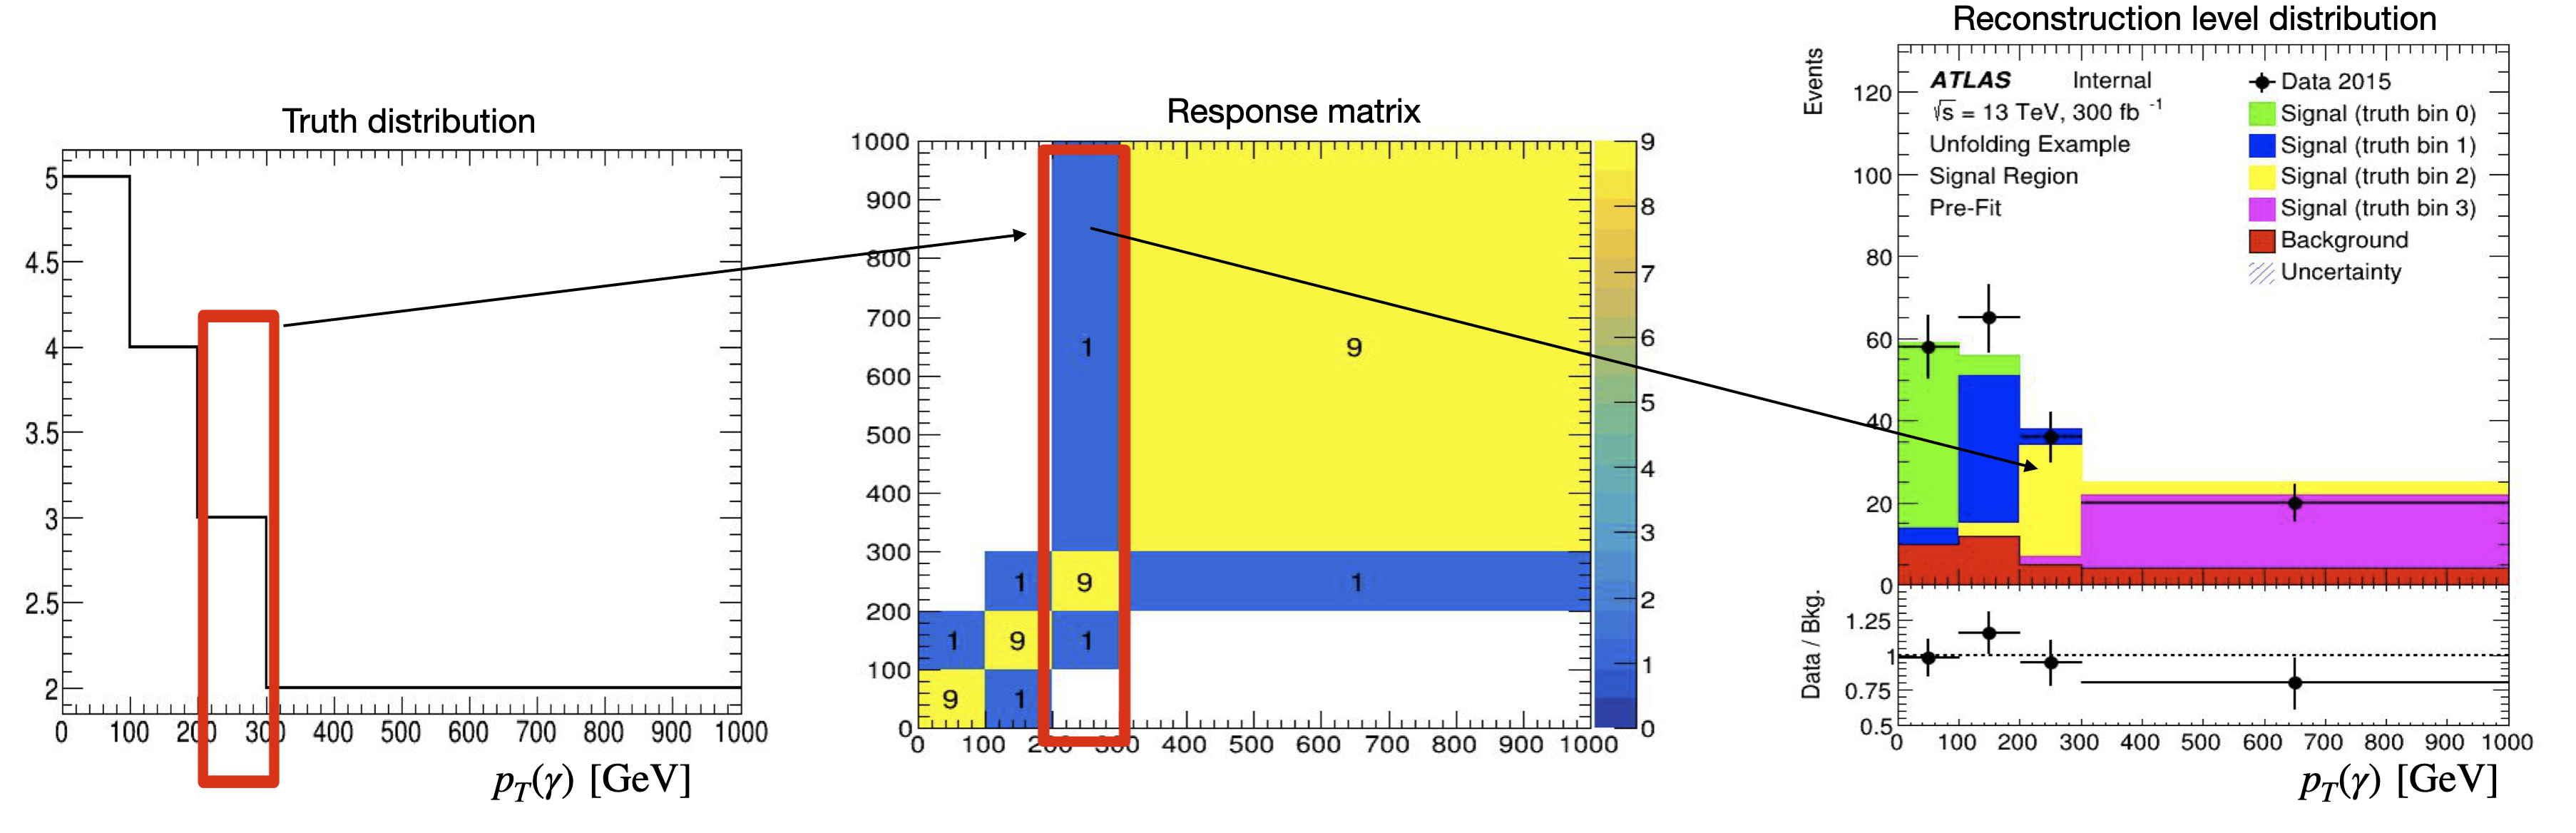
\includegraphics[width=0.9\textwidth]{figures/toy_profile_likelihood_fit.png}
    \caption{Toy example to illustrate the unfolding procedure. The truth distribution is multiplied by the response matrix to obtain the distribution at the reconstruction level. A normalization factor is assigned for each bin of the truth distribution. Profile likelihood fit is performed to the reconstruction level distribution to obtain the normalization factors. The truth distribution is directly obtained from the normalization factors.}

    \label{fig:unfolding_toy_example}
\end{figure}
\FloatBarrier

The likelihood is constructed using the signal and background templates in the following way:
\begin{equation}\label{eq:likelihodd-defn}
	L(\vec{n}^{data} | \vec{k}, \vec{\theta}) = \prod_{\mathrm{c} \epsilon \mathrm{Region}} \quad \prod_{\mathrm{b} \epsilon \mathrm{Bins}} \mathrm{Pois} (n^{\mathrm{data}}_{b,c}|\nu_{b,c}(\vec{k}, \Vec{\theta})) \cdot \prod_{p} \mathrm{Gauss}(0|\theta_{p},1)
\end{equation}

where, \textit{Region} refers to the different signal and control regions, \textit{Bins} refers to the bin of the reconstruction level histogram, $n^{\mathrm{data}}_{b,c}$ is the data in bin \textit{b} and region \textit{c}, $\nu_{b,c}$ is the expected total events in bin \textit{b} and channel \textit{c}. $\Vec{\theta}$ are the constrained nuisance parameter describing systematic uncertainties \cref{sec:sources-of-uncertainties} and $\mathrm{Gauss}(0|\theta_p,1)$ is a Gaussian constraint of the NP $\theta_p \in \vec{\theta}$ with mean of 0 and standard deviation of 1, $\vec{k}$ are the unconstrained parameters (e.g. POIs).

$\nu_{b,c}$ can be expressed as follows:

\begin{align}\label{eq:likelihodd-defn-1}
    \nu_{b,c} = \left[\sum_i \gamma_{b,c,i} \cdot \mu_{i} \cdot R_{b,c,i} \cdot T_{i}\right] + \sum_{B} \gamma_{b,c}^{B} \times N_{b,c}^{B} 
\end{align}

where, $\gamma$ factors are the bin-by-bin scale factors for MC statistical uncertainties. The background samples each have the factors $\gamma_{b,c}^{B}$ and for the signal, each truth bin has a unique $\gamma_{b,c,t}$. $R_{b,c,t}$ are the response matrices of the signal, calculated from the particle level and reconstruction level events. $\mu_{i}$ corresponds to the signal strength of the bin $T_{i}$ at particle level.

Subsequently, a Profile Likelihood fit is performed with this Likelihood in \emph{TRexFitter}\footnote{\url{https://trexfitter-docs.web.cern.ch/trexfitter-docs/}}.

% mention the later story, the minimization and so on.
% put more details on the fit and unfolding?
% Also how the uncertainties are taken into account in the likelihood function
% with which errors are calculated also

